%% Copernicus Publications Manuscript Preparation Template for LaTeX Submissions
%% ---------------------------------
%% This template should be used for copernicus.cls
%% The class file and some style files are bundled in the Copernicus Latex Package, which can be downloaded from the different journal webpages.
%% For further assistance please contact Copernicus Publications at: production@copernicus.org
%% https://publications.copernicus.org/for_authors/manuscript_preparation.html

\documentclass[soil, manuscript]{copernicus}

%% \usepackage commands included in the copernicus.cls:
%\usepackage[german, english]{babel}
%\usepackage{tabularx}
%\usepackage{cancel}
%\usepackage{multirow}
%\usepackage{supertabular}
%\usepackage{algorithmic}
%\usepackage{algorithm}
%\usepackage{amsthm}
%\usepackage{float}
%\usepackage{subfig}
%\usepackage{rotating}

% *** comment this out before submission and remove or comment out any notes
% *** To comment, use the \verb=\todo[inline]{YourInitials: comment}= command.
\usepackage{todonotes}

\usepackage{natbib}

\begin{document}

\title{How well do digital soil maps represent ``reality''?}

% \Author[affil]{given_name}{surname}

\Author[1,2]{D G}{Rossiter} %% correspondence author
\Author[1]{Laura}{Poggio}

\affil[1]{ISRIC-World Soil Information, Wageningen (NL)}
\affil[2]{Section of Soil \& Crop Sciences, College of Agriculture \& Life Sciences, Cornell University, Ithaca NY 14850 (USA)}

\correspondence{D G Rossiter (david.rossiter@isric.org)}


\runningtitle{DSM vs. ``reality''}

\runningauthor{D G Rossiter}

\received{}
\pubdiscuss{} %% only important for two-stage journals
\revised{}
\accepted{}
\published{}

%% These dates will be inserted by Copernicus Publications during the typesetting process.

\firstpage{1}

\maketitle
\tableofcontents

\newpage
\begin{abstract}
 %
Any map should be a faithful representation of what it is designed to show, with some generalization appropriate to the map scale or grid cell resolution.
%
Maps of soil properties should thus correspond to the actual vertical and horizontal distribution of soil properties on the ground.
%
Similarly, maps of soil types should correspond to the actual types, according to the central concept and property range of each type.
%
Digital soil maps (DSM) predict at grid cells either as point or block estimates, but the evaluation must be of the patterns over the mapped area, including spatial concepts such as connectivity, adjaceny, and form.
%
This is intrinsically connected with the concepts of map scale, grid cell resultion, categorical and cartographic detail.
\end{abstract}

\newpage
\introduction  %% \introduction[modified heading if necessary]

\par
Digital Soil Mapping (DSM) is now the dominant method of making new soil maps.
%
DSM consists of training a model (either geostatistical or machine learning) on known observations, using their location and (for machine learning models) values of covariates at these locations.
%
The model is then applied over an area to be mapped, either by interpolation, by application of the machine-learning model, or a combination, to make a predictive map with quantified uncertainty at each location, typically a grid at some horizontal resolution.

\par
How useful are these maps? One answer is the per-grid cell evaluation of uncertianty, compared to acceptance criteria for one or more uses.
%
However, many uses require knowledge of the soil pattern, not just at individual points.
%
Except for precision agriculture, land is managed as units of more or less homogeneous soils, or at least a consistent pattern of contrasting soils.
%
Hydrologic models require connectivity between grid cells, as water flows over or through the landscape.

\section{What is ``Reality''?}

\par
Point-wise reality is the actual vertical distribution of a set of soil properties at pedon scale.
%
These are levels \textit{i} (pedon) and \textit{i-1} (horizon) of \citet{Hoosbeekquantitativemodelingpedogenesis1992}'s organizational hierarchy.
%
Finer scales are not mapped.

\subsection{Vertical reality}

DSM predicts soil properties either pointwise at fixed depths, or as averages over a fixed depth slice.
%
By far the most common set of depths are those specified by the GlobalSoilMap project \citep{ScienceCommittee2015a}: 0-5, 5-15, 15-30, 30-60, 60-100, 100-200~cm.
%
These were chosen to provide a reasonable resolution for land surface modelling.
%
This contrasts with the organization of natural soil bodies as pedogenetic horizons, which are the usual vertical resolution units in field descriptions and laboratory analyses.
%
The horizons are separated by boundaries that range from very sharp to diffuse, as recognized in field description manuals \citep{usdanaturalresourcesconservationservice.FieldBookDescribing2024, foodandagricultureorganizationoftheunitednationsGuidelinesSoilDescription2006}.
%
No DSM method to date recognizes different thickness of transition.
%
This could be partially offset by predicting at many thin depth slices, but this would require similarly fine-resolution training profile sampling, or else inferring transition horizons from the sampled genetic horizons and horizon boundary descriptions.

\par
So the correspondence with vertical ``reality'' is reduced to accuray of either the value at the depth slice centre, or its mean over the depth slice.
%
Whether this is sufficient for a given application can not be assessed.

\subsection{Horizontal reality}
%

\par
The reality over areas includes the relation between pedons, i.e., polypedons of similar and contrasting soils \citep{johnsonPedonPolypedon1963}.
%
The DSM product should show these relations.
%

\subsubsection{Soil property  maps}

DSM typically predicts a  large number of soil properties (either primary or derived by pedotransfer functions) at a series of standardized depth slices.
%
Some properties have a clear landscape relation, whereas others are more related to internal organization of the soil body.
%
Examples of the first case are particle-size class in an alluvial landscape, or 

\subsubsection{Soil class maps}

\par
DSM can also be used to predict soil classes at each grid cell, either at its centre or as the dominant class in a cell.
%
Most DSM methods can predict the probability of occurrence of one or more classes; an example is the probability forest implemented in the \texttt{ranger} R package \citep{Wright.Ziegler2017}.
%
Of course, in a closed classification system a pedon can only be assigned to one class, so that the most probable class is typically presented, along with its uncertainty evaluated by the Brier score, entropy, or a confusion index.
%
Pointwise or grid cell-wise  accuracy is evaluated with confusion matrix statistics \citep{CongaltonAssessingaccuracyremotely2009}.
%
However, this does not account for spatial patterns of soil classes.
%
The concept of the polypedon (contiguous group of pedons of the same class) show that the DSM-produced pattern must be evaluated again the actual pattern of polypedons.

\par
Although we never know the complete pattern, soil class maps made by expert landscape analysis and field investigation show discrete map delineations with a minimum ground area corresponding to the design scale.
%
These maps are made according to the soil survey landscape analysis paradigm \citep{hudsonSoilSurveyParadigmbased1992}, based primarily on objective information (landforms, land use) informing tacit knowledge and expert judgement.
%
So one test of DSM is how closely it matches traditional soil class maps, at the same categorical and cartographic detail.

\par
Each delineation is part of a map unit (also called a legend category), linked to a description of the range of soil classes, typical soil profiles, and associated laboratory analysis to be found within the map unit. The legend is either local names for a soil type or group of them, or a name within a soil classification system.
%
Figure \ref{fig:pq49b3} shows a typical example from Qu\'{e}bec \citep{grenonEtudePedologiqueComte1999}.
%
Map units in this example are named for a soil series, the dominant soil texture, soil thickness, and local terrain form.
%
The series name is linked to a modal profile and limits for the horizons and the various properties measured for each.
%
The delineations show an obvious pattern, which the survey has inferred from landscape analysis.
%
Fluvial systems, contrasting parent materials, and geologic structures are clearly visible.
%
Other boundaries are not obviously linked to the landscape, but may have been inferred from depositional history discovered in the field land use preferences.
%
In any case we would like the DSM to represent these units, perhaps with more precise boundary placement due to precisely georeferenced covariates, and perhaps with some boundaries as transition zones \citep{LagacherieFuzzinessuncertaintysoil1996}.

\begin{figure}
  \centering
  \includegraphics[width=\textwidth]{pq49b_map_3_part.jpg}  
  \caption{A portion of typical semi-detailed soil class map. Source \citep{grenonEtudePedologiqueComte1999}}
  \label{fig:pq49b3}
\end{figure}

\par
DSM predicts over grid cells much larger than a pedon.
%
Geostatistical methods can predict averages their uncertainties over a block the size of the grid cell, but the average is not observed in the field (unless the entire grid cell would be dug up for examination!).
%
Machine-learning methods predict at the same support as the training observations, i.e., ``point'' (pedon) support, and the predicted values and their uncertainties are implicity extended to the whole grid cell.
%
So here the reality is the average -- any finer-scale detail of reality is by definition not representable by this DSM.

\section{Concepts of spatial organization}

\par
The categorization spatial pattern of soil bodies was extensively studied over 50 years ago, notably by \citet{Fridland1972,Fridland1974} and \citet{holeApproachLandscapeAnalysis1978, holeSoilLandscapeAnalysis1985}.
%
Fridland defined ``soil combinations'', whereas Hole used the term ``soilscape fabrics''.
%

\subsection{Fridland's concepts}

\par
\citet{Fridland1974} explains that ``\emph{[s]oil combinations} consist of elementary soil areas which are \emph{genetically linked} to various degrees and which produce a \emph{definite pattern} in the soil mantle
%
\ldots
%
Multiple spatial repetition of a certain soil combination or several soil combinations alternating in a definite order creates various forms of structures of the soil mantle
%
\ldots
%
The initial indivisible component of the soil mantle is the \emph{elementary soil area} which represents a body of soil that belongs to a certain classificational unit of the lowest rank and occupies space which is bounded on all sides by other elementary soil areals or non-soil formation'' (emphasis added).

\par
At the finest scale these are:

\begin{enumerate}
\item[0.] Homogeneous;
\item Sporadically spotted: ``minute'' areas of contrasting soils: e.g., from tree throw, termite mounds,  carbonate solution-driven  depth of pedogenesis;
-- can be found by comprehensive geotechnical investigation or precision ag. technology; these DSM are not considered here;
\item Regular-cycling: e.g.,  gilgai;
\item apparent diffusion.
\end{enumerate}

The sporadically spotted scale can not be captured by any reasonable DSM scale.

He then defines local patterns related to geomorphic process, parent material, or pedologic processes:

\begin{enumerate}
\item Dendritic, linear-dendritic and streaming forms, connected with various forms of the erosional relief;
\item  Rounded-spotted (including ringlike) forms, connected with various depressional forms (sink holes, depressions of different types and lakes) and hilly-morainic relief;
\item  Linear and wavy-linear forms connected with different linear forms of relief of an accumulative and somewhat erosional origin;
\item  Streak-phacoid forms (referring to \emph{Phacoides} bivalve shells)  characteristic of modern and ancient flood plains and deltas;
\item  A fan-shaped genetic and geometric structure is characteristic of alluvial fans and proluvial--deluvial trains;
\item A geometrically disordered structure of the soil mantle is usually conditioned by the heterogeneity of the soil-forming rocks and their irregular succession.
\end{enumerate}

If these local patterns are at sufficiently coarse size to be represented at the DSM resolution, we should see them on the DSM map.

\subsection{Hole's concepts}

\citet{holeSoilLandscapeAnalysis1985} relates the \emph{pedologic fabric} of the landscape in terms of the size, shape and arrangement of bodies of soil and associated not-soil.
%
These are all called \emph{associations}, depending on the size of mapping units on a polygon map of soil bodies.

\par
\citet[Table 5]{holeApproachLandscapeAnalysis1978} first discusses sizes of map units.
%
The soil individuals of map units as they exist on the ground are of size $\approx 1 \mathrm{m}^2$; this is the pedon.
%
These then can be grouped into polypedons:
%
\begin{enumerate}
\item Micro: $<0.1 \; \mathrm{ha}$;
\item Meso: $0.1 - 1.0 \;\mathrm{ha}$;
\item Macro: $10 - 100 \; \mathrm{ha}$;
\item Mega: $>100 \; \mathrm{ha}$;
\end{enumerate}
%

\par
Figure \ref{fig:hole12} shows how soil bodies can be delineated at increasingly fine scale, depending on the categorical degree of contrast between them.

\begin{figure}
  \centering
  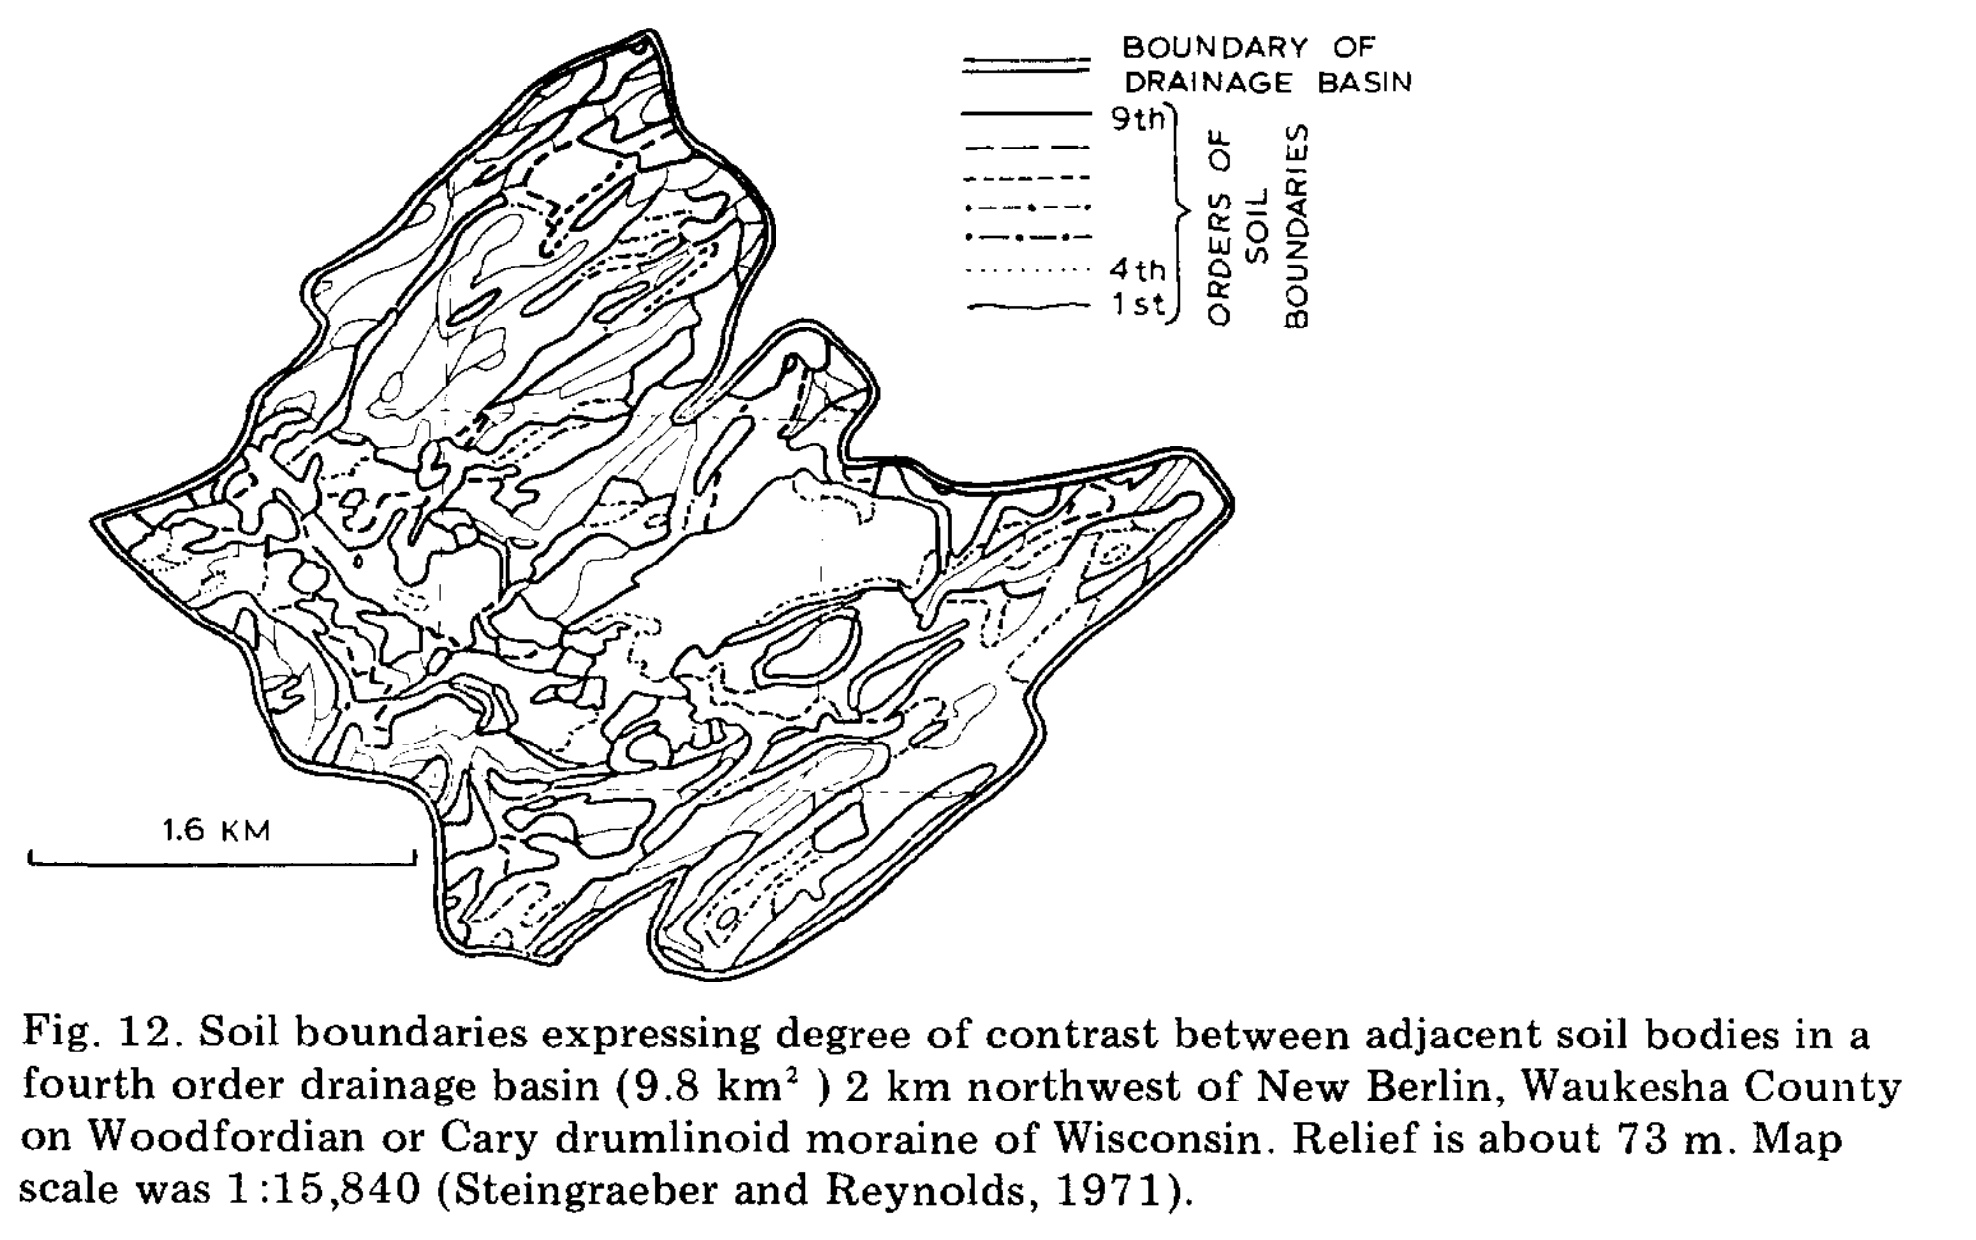
\includegraphics[width=0.45\textwidth]{10.1016.0016-7061(78)90002-2_Fig12.png}
  \hfill
  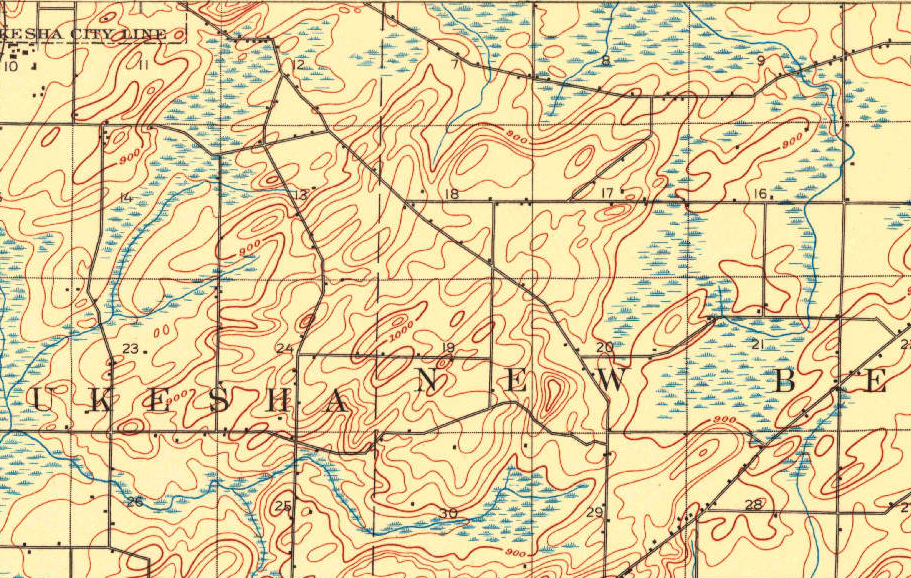
\includegraphics[width=0.45\textwidth]{10.1016.0016-7061(78)90002-2_Fig12_topo1901.png}
  \caption{Orders of soil boundaries. Left: Figure 12 from \citep{holeApproachLandscapeAnalysis1978}; Right: topography of this area, USGS topographic map 1901.}
  \label{fig:hole12}
\end{figure}


\par
Over larger extents, \citet[Table 5]{holeApproachLandscapeAnalysis1978} identifies:
%
``microassociation'' mapping units have size $<250 \; \mathrm{km}^2$;
%
``mesoasociation'' mapping units $250-2~500 \; \mathrm{km}^2$; and
%
``macroasociation'' mapping units  $2~500 - 250~000 \;\mathrm{km}^2$.
%
``megaasociation'' mapping units  $> 250~000 \; \mathrm{km}^2$.
%
These scales are not relevant to the current discussion.

\par
\citet[Figure 5]{holeApproachLandscapeAnalysis1978}  then discusses general categories of shapes of soil bodies:
\begin{enumerate}
\item disks
\item spots
\item stripes (simple or branched)
\item categorized by shape index (boundary length divided by periphery of a circle of the same area) as simple to rounded, and complex to angular.
\end{enumerate}
%
These can be identified at any resolution, depending on the spatial arrangement of the soil-forming process.


\section{Patterns represented by DSM}

\par
Different DSM methods are capable of represent different patterns:

\begin{itemize}
\item Trend surfaces, including polynomial trends, thin-plate splines (TPS) and generalized additive models (GAM): These can represent smooth transitions over local to wide areas.  Splines and GAM show both in one model.
\item Interpolation by pure geostatistics, e.g., Ordinary Kriging (OK): These show smooth local transitions in the neighbourhood of training points. Thus they are well-suited to ``spots'' or ``disks''.
\item Tree-based or neural network-based machine learning: These predict separately at each grid cell, based on the trained model. There is no requirement for spatial continuity.  This allows finely-speckled patterns of contrasting soils -- whether these are realistic or not.
\end{itemize}

\section{What is predicted by DSM?}

DSM predicts separately at each grid cell. The prediction can be of different supports:

\begin{enumerate}
\item at the centre point as a single predicted value, implicitly at the point-support size of the training data. This is typical of ML predictions.
  %
  The value is then supposed to be uniform within the grid cell, at any point support within it.
%
  The grid cell size is limited by finest-resolution covariate.
  %
  There is no information at finer resolution.
  %
  This accounts for possible imprecise georeferencing within the grid cell size.
  %
  The covariate values at this grid cell size may be integrations of all values. This is typical of remote sensing pixels with a defined field of view, and receiving energy from that entire field.
  %
  Other covariate values may be ``point'' predictions, also referenced to the grid cell centre. An example is an predicted climate surface interpolated from point observations.
  %
\item over the pixel as a mean value, also from point-support training data. This can be accomplished by block kriging.
\end{enumerate}


\section{Scale and resolution}

\par
The level of detail on a map has two components: categorical and cartographic.
%
Categorical detail is the precision of information. For a continuous variable it is the measurement precision.
%
For ordinal categorical variables generalized from continuous variables it is the class width.
%
For nominal categorical variables based on classes, e.g., a soil classification system, it is the extent of properties of the class.
%
This latter is implicit in monothetic hierarchical soil classification systems, notably USDA Soil Taxonomy, but also the World Reference Base for Soil Classification and many national systems.

\par
The resolution of the DSM product dictates which of these can be identified on the DSM map.
%
Table 1 in \citep{mcbratneyDigitalSoilMapping2003} presents a link between soil survey orders, as defined by the USDA NRCS, scale, and resolution.
%
The equivalent map scale is determined by assuming a  $1 \times 1 \; \mathrm{mm}$ paper map area as the smallest discernible area, so that the scale is $1 \; \mathrm{m}/1000 s$, where $s$ is the side length of 1000 grid cells.
%
For example with 250~m horizontal resolution grid cells, this is $1:250~000$ (reconaissance or general soil survey, order 4/5); for 30~m  grid cells this is $1:30~000$ (semi-detailed soil survey, order 2/3).
%
These authors further argue that, because of the Nyquist frequency, in fact a $2 \times 2$ grid cell block must be considered the minimum unit in a DSM, so the effective resolution is twice the nominal resolution.
%
So in these two examples the effective equivalent map scale would be $1:500~000$ (order 5) and $1:60~000$ (order 3).
%
The minimum legible delineation (MLD) for a DSM product is thus four grid cells, and any variation within is by definition ``noise'' which can't be evaluated.

\par
Implicitly the DSM represents the class or value as uniform within the MLD.

\section{Case studies}

In this section we examine some interesting soil patterns from different parts of the world, and see how DSM products reproduce these.

\subsection{Case Study -- Kenya}

iSDA maps vs.\ colonial maps, see \emph{/Users/rossiter/Library/Mobile Documents/com~apple~CloudDocs/Documents/data/Journal/BookChapters/DSM2006/graph}. We should see the ironstone hills (coarse fragments), river valley (silt) etc.

\subsection{Case Study -- European soil classes}

WRB Reference Soil Groups with one principal classifier were mapped over Europe by  Miniak\url{https://zenodo.org/records/13838408}.


\subsection{Case Study -- Central New York (USA) drumlin field}

\citep{naumanSoilLandscapesUnited2024}

\subsection{Case Study -- Missippi Delta alluvial plain}

\par
The Missipppi River has created a wide plain of active and abandoned channels, backswamps, levees, and terraces.
%
In the State of Mississippi this is referred to as the ``Delta''.
%
This creates a clear pattern of particle-size classes.
%
Figure \ref{fig:stovall} shows a typical pattern.

\begin{figure}
  \centering
  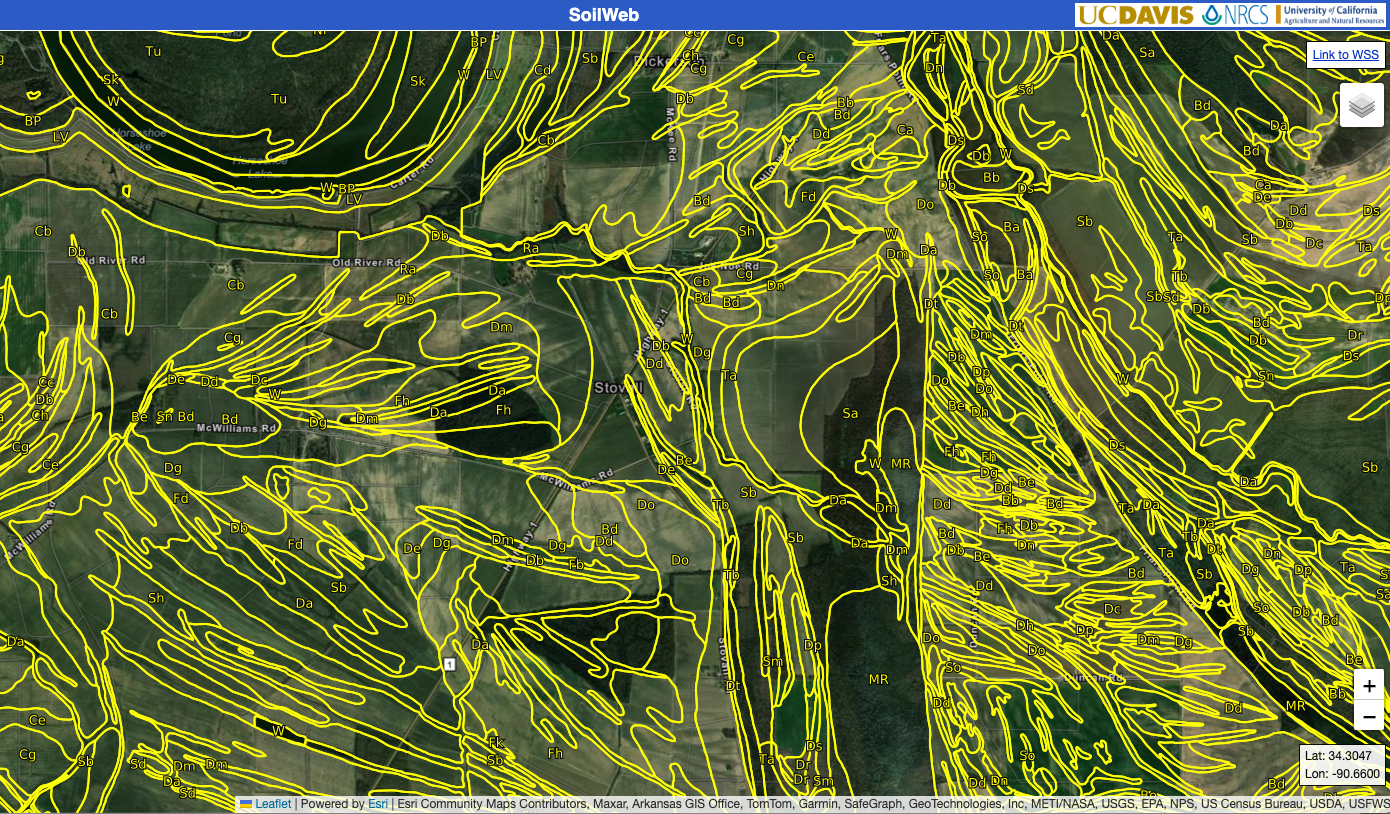
\includegraphics[width=\textwidth]{SoilWeb_StovallMS.png}
 \caption{Soil series map, centred at Stovall (MS).}
  \label{fig:stovall}
\end{figure}



\subsection{Case Study -- Driftless area of Wisconsin (USA)}

Soil series of the Raffelson  area in the Driftless Area of Wisconsin has extensively mapped with the SolIM approach \citep{Zhu.etal2001,zhuPredictionSoilProperties2010}.
%
This area has a regular topography with typical landscape positions for each soil series.




%%%%%%%%%%%
\conclusions[Discussion]  %% \conclusions[modified heading if necessary]
%
Final discussion and recommendations for DSM assessment.



%\codedataavailability{}


%\appendix
%\section{}    %% Appendix A

%\subsection{}     %% Appendix A1, A2, etc.

%\noappendix       %% use this to mark the end of the appendix section. Otherwise the figures might be numbered incorrectly (e.g. 10 instead of 1).

%% Regarding figures and tables in appendices, the following two options are possible depending on your general handling of figures and tables in the manuscript environment:

%% Option 1: If you sorted all figures and tables into the sections of the text, please also sort the appendix figures and appendix tables into the respective appendix sections.
%% They will be correctly named automatically.

%% Option 2: If you put all figures after the reference list, please insert appendix tables and figures after the normal tables and figures.
%% To rename them correctly to A1, A2, etc., please add the following commands in front of them:

%\appendixfigures  %% needs to be added in front of appendix figures

%\appendixtables   %% needs to be added in front of appendix tables

%% Please add \clearpage between each table and/or figure. Further guidelines on figures and tables can be found below.

\authorcontribution{DGR conceived of the ideaand wrote the initial draft. LP contributed advice at every step, especially the concepts and interpretations.} %% this section is mandatory

\competinginterests{The authors have no competing interests} %% this section is mandatory even if you declare that no competing interests are present

% \disclaimer{TEXT} %% optional section

%\begin{acknowledgements}
%TEXT
%\end{acknowledgements}


%% REFERENCES

%% The reference list is compiled as follows:

%% Since the Copernicus LaTeX package includes the BibTeX style file copernicus.bst,
%% authors experienced with BibTeX only have to include the following two lines:
%%
\addcontentsline{toc}{section}{References}
\bibliographystyle{copernicus}
\bibliography{reality.bib}

%% URLs and DOIs can be entered in your BibTeX file as:
%%
%% URL = {http://www.xyz.org/~jones/idx_g.htm}
%% DOI = {10.5194/xyz}


%% LITERATURE CITATIONS
%%
%% command                        & example result
%% \citet{jones90}|               & Jones et al. (1990)
%% \citep{jones90}|               & (Jones et al., 1990)
%% \citep{jones90,jones93}|       & (Jones et al., 1990, 1993)
%% \citep[p.~32]{jones90}|        & (Jones et al., 1990, p.~32)
%% \citep[e.g.,][]{jones90}|      & (e.g., Jones et al., 1990)
%% \citep[e.g.,][p.~32]{jones90}| & (e.g., Jones et al., 1990, p.~32)
%% \citeauthor{jones90}|          & Jones et al.
%% \citeyear{jones90}|            & 1990



%% FIGURES

%% When figures and tables are placed at the end of the MS (article in one-column style), please add \clearpage
%% between bibliography and first table and/or figure as well as between each table and/or figure.

% The figure files should be labelled correctly with Arabic numerals (e.g. fig01.jpg, fig02.png).


%% ONE-COLUMN FIGURES

%%f
%\begin{figure}[t]
%\includegraphics[width=8.3cm]{FILE NAME}
%\caption{TEXT}
%\end{figure}
%
%%% TWO-COLUMN FIGURES
%
%%f
%\begin{figure*}[t]
%\includegraphics[width=12cm]{FILE NAME}
%\caption{TEXT}
%\end{figure*}
%
%
%%% TABLES
%%%
%%% The different columns must be seperated with a & command and should
%%% end with \\ to identify the column brake.
%
%%% ONE-COLUMN TABLE
%
%%t
%\begin{table}[t]
%\caption{TEXT}
%\begin{tabular}{column = lcr}
%\tophline
%
%\middlehline
%
%\bottomhline
%\end{tabular}
%\belowtable{} % Table Footnotes
%\end{table}
%
%%% TWO-COLUMN TABLE
%
%%t
%\begin{table*}[t]
%\caption{TEXT}
%\begin{tabular}{column = lcr}
%\tophline
%
%\middlehline
%
%\bottomhline
%\end{tabular}
%\belowtable{} % Table Footnotes
%\end{table*}
%
%%% LANDSCAPE TABLE
%
%%t
%\begin{sidewaystable*}[t]
%\caption{TEXT}
%\begin{tabular}{column = lcr}
%\tophline
%
%\middlehline
%
%\bottomhline
%\end{tabular}
%\belowtable{} % Table Footnotes
%\end{sidewaystable*}
%
%
%%% MATHEMATICAL EXPRESSIONS
%
%%% All papers typeset by Copernicus Publications follow the math typesetting regulations
%%% given by the IUPAC Green Book (IUPAC: Quantities, Units and Symbols in Physical Chemistry,
%%% 2nd Edn., Blackwell Science, available at: http://old.iupac.org/publications/books/gbook/green_book_2ed.pdf, 1993).
%%%
%%% Physical quantities/variables are typeset in italic font (t for time, T for Temperature)
%%% Indices which are not defined are typeset in italic font (x, y, z, a, b, c)
%%% Items/objects which are defined are typeset in roman font (Car A, Car B)
%%% Descriptions/specifications which are defined by itself are typeset in roman font (abs, rel, ref, tot, net, ice)
%%% Abbreviations from 2 letters are typeset in roman font (RH, LAI)
%%% Vectors are identified in bold italic font using \vec{x}
%%% Matrices are identified in bold roman font
%%% Multiplication signs are typeset using the LaTeX commands \times (for vector products, grids, and exponential notations) or \cdot
%%% The character * should not be applied as mutliplication sign
%
%
%%% EQUATIONS
%
%%% Single-row equation
%
%\begin{equation}
%
%\end{equation}
%
%%% Multiline equation
%
%\begin{align}
%& 3 + 5 = 8\\
%& 3 + 5 = 8\\
%& 3 + 5 = 8
%\end{align}
%
%
%%% MATRICES
%
%\begin{matrix}
%x & y & z\\
%x & y & z\\
%x & y & z\\
%\end{matrix}
%
%
%%% ALGORITHM
%
%\begin{algorithm}
%\caption{...}
%\label{a1}
%\begin{algorithmic}
%...
%\end{algorithmic}
%\end{algorithm}
%
%
%%% CHEMICAL FORMULAS AND REACTIONS
%
%%% For formulas embedded in the text, please use \chem{}
%
%%% The reaction environment creates labels including the letter R, i.e. (R1), (R2), etc.
%
%\begin{reaction}
%%% \rightarrow should be used for normal (one-way) chemical reactions
%%% \rightleftharpoons should be used for equilibria
%%% \leftrightarrow should be used for resonance structures
%\end{reaction}
%
%
%%% PHYSICAL UNITS
%%%
%%% Please use \unit{} and apply the exponential notation


\end{document}
